\documentclass[12 pt]{article}
\usepackage{amsmath}
\usepackage{url}
\usepackage{graphicx}
\usepackage{setspace}
\usepackage{pgf}
\usepackage{tikz}
\usetikzlibrary{arrows,automata}
\usepackage[latin1]{inputenc}
\usepackage{verbatim}
\usepackage{lscape}
%\usepackage[margin=1.2in]{geometry}

	\addtolength{\oddsidemargin}{-.5in}
	\addtolength{\evensidemargin}{-.5in}
	\addtolength{\textwidth}{0.75in}
	\addtolength{\topmargin}{-1in}
	\addtolength{\textheight}{1.75in}
\begin{document}

\newcommand{\vocab}{\mathbf{v}}
\newcommand{\dtvec}{\mathbf{t}_\Delta}
\newcommand{\ctxvec}{\mathbf{t}_\text{ctx}}
\newcommand{\dt}{\Delta_t}


\section{Method}

Extract data collected from forums Timestamp, Author, Text Content. Using sliding window training method, group consecutive $w$ posts together and perform regression on $\Delta_t$. More formally, we are trying to learn a function $f$ such that $f(\mathbf{x}_{t-w},\hdots, \mathbf{x}_{t-1}) \approx \Delta_{t}$, where $\mathbf{x}_t$ is a post made at time $t$, and $\Delta_t$ is the time between the $t$-th post and the $(t-1)$-th post. The following are the features used:
\begin{description}
	\item[Previous time differences] All the time differences between posts made in the window. ($\mathbf{t}_\Delta$)
	\item[Time-based features] Day of week, Hour of day. Provides contextual information about when the post was made. ($\mathbf{t}_{\text{ctx}}$)
	
	\item[Content features (text)] Word frequency counts. Used regression to test effect of single regressor. Top $F$ features are selected for extraction. ($\mathbf{w}$)

\end{description}

%include diagrams

\subsection{Evaluation metrics}
We use \emph{Mean Absolute Percentage Error} (MAPE), to measure the performance of the learnt model. This value is given by
\[
	\frac{1}{N}\sum^N_{i=1}\left|\frac{A_i-F_i}{A_i}\right|
\]
where $A_i$ is the actual value, and $F_i$ is the forecasted value for the instance $i$. Realistically, the model would not be able to come into contact with every possible window, since chances are it will make an error that causes %explain error in a new section (before this one) ?
it to visit a thread late, causing it to miss two posts or more. This value does not reflect how well the model will do in a real-time setting, but gives an idea of how far off the model is given a window. 

We also want to know the \emph{timeliness} of the model's visits. Yang et. al. \cite{Yang2009} has a metric for measuring this. Taking $\Delta t_i$ as the time difference between a post $i$ and it's download time, the timeliness of the algorithm is given by
\[T = \frac{1}{N} \sum^{N}_{i=1}\Delta t_i\]
A good algorithm would give a low $T$-score. However, a crawler that hits the site repeatedly performs well according to this metric. The authors account for this by setting a bandwidth (fixed number of pages per day) for each iteration of their testing. This will contribute to the $T$ value when such a naive crawler uses up its daily bandwidth and can only resume its downloading the next day.

Viewing the posts made during the thread's lifetime as segmentations of the thread, and the visits made as hypotheses of where the segmentations are, we use the $Pr_{error}$ metric from Georgescul et. al. , 2006 as a measure of how close the predictions are to the actual posts.



\section{Results}

The results for experiments done with different combinations of the above specified features are shown in Table \ref{expt1}.
\begin{table}
	\footnotesize
	\begin{centering}
	\begin{tabular}{|l|c|c|c|c|c|c|c|c|}
	\hline
	\input{init_res}
	\hline
	\end{tabular}
	\caption{Experiment results}
	\label{expt1}
\end{centering}
\end{table}

Overall average and window average perform very poorly, on MAPE score, reflected in $T$-score.

Looking at $T$-score and no. of visits together, would seem that $\textbf{t}_\Delta$ is important feature (Including reduces $T$-score).

Using content (word frequency) features for prediction, gives only slight improvement.

High values for $Pr_{miss}$ and low for $Pr_{fa}$, are due to

	Mainly due to $Pr_{miss}$ being conditioned on the fact that there must be a segmentation/post there.
	Posts come in bursts, visits are fairly periodic, and intervals between visits are larger than post bursts.
	More posts than visits in places with posts, hence higher $Pr_{miss}$

	High no. of invalid predictions.
\begin{landscape}
\begin{figure}
	\centering
	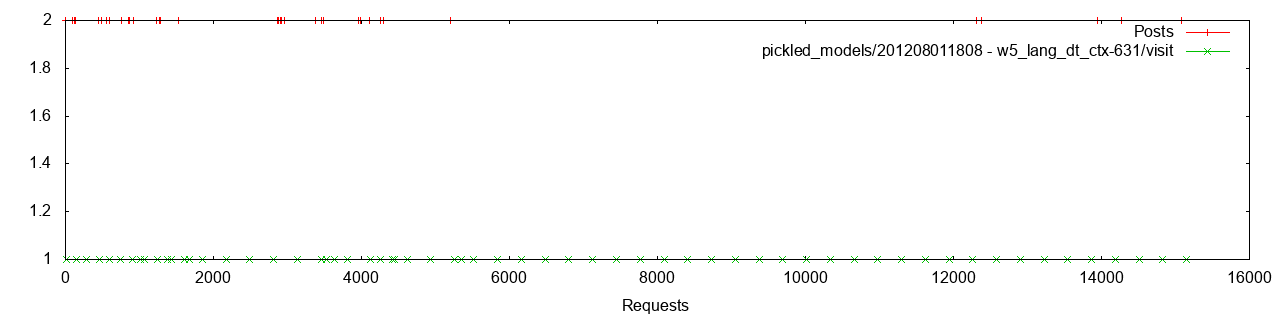
\includegraphics[scale=0.5]{example_seq.png}
	\caption{Visitation chart for a model using the $w=5, \mathbf{t}_\Delta, \mathbf{t}_{\text{ctx}},\mathbf{w}$ feature set. Invalid Predictions = 0.758, $Pr_{error} =  0.485$, $T$-score = 119.612, Posts = 41, Visits = 62}
\end{figure}
\end{landscape}

\begin{table}
	\footnotesize
	\begin{centering}
	\begin{tabular}{|l|c|c|c|c|c|c|c|c|}
	\hline
	\input{f_size}
	\hline
	\end{tabular}
	\caption{Experiment results: Varying feature sizes}
	\label{expt1}
\end{centering}
\end{table}

\begin{table}
	\footnotesize
	\begin{centering}
	\begin{tabular}{|l|c|c|c|c|c|c|c|c|}
	\hline
	\input{vocab_exp}
	\hline
	\end{tabular}
	\caption{Experiment results: Varying vocabulary size}
	\label{expt1}
\end{centering}
\end{table}


\

\bibliographystyle{acm}
\bibliography{report}
\end{document}
